\documentclass[border=10pt]{standalone}
\usepackage{pgfplots}
\pgfplotsset{compat=1.18}
\begin{document}
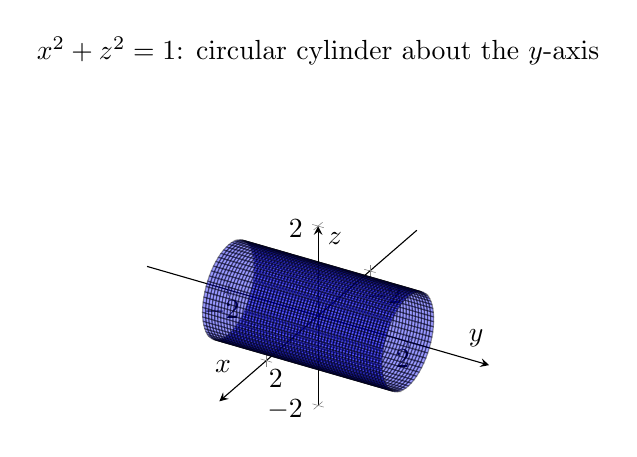
\begin{tikzpicture}
\begin{axis}[
    view={120}{30},
    xlabel={$x$}, ylabel={$y$}, zlabel={$z$},
    xmin=-2, xmax=2, ymin=-2, ymax=2, zmin=-2, zmax=2,
    axis equal,
    axis lines=center,
    samples=60, samples y=60,
    title={$x^2+z^2=1$: circular cylinder about the $y$-axis}
]
\addplot3[surf, domain=0:360, y domain=-2:2, z buffer=sort,
    variable=\u, variable y=\v,
    color=blue, opacity=0.4, faceted color=black]
({cos(u)}, {v}, {sin(u)});
\end{axis}
\end{tikzpicture}
\end{document}
